\section{Detection sensitivity with Advanced gravitational wave detectors}
\label{sec:results}

To estimate how accurately we can infer the time evolution of $r=M_{\rm PNS}/R_{\rm PNS}^2$ in the
gravitational wave detector data, we have added {\texttt s20S} GW signal to 
100 Gaussian noise realisations whose power spectral density follows advanced LIGO (aLIGO)
spectrum~\cite{aLIGOsens:2018} shown on Figure~\ref{fig:spectrum}. 
We have varied the distance to the source, covering a large
range of distances for which a detection in second generation of gravitational wave detectors
is feasible. The source is optimally oriented with
respect to the gravitational wave detector. We are assuming a GW signal from a core collapse
phenomena has been identified in the data and that the beginning of the GW signal is known within $O(10~ms)$.
The data (signal embedded in noise) are whitened using the function {\it prewhiten} of the R-package TSA.
An auto-regressive model with maximal \textcolor{red}{100} coefficients has been used.    

For each of the noise realisations, we reconstruct the ratio time series {$r_i$}
of length $N$ and compare it to ratio {$r_i^0$} derived from
the PNS mass and radius generated by the simulation code that produced {\texttt s20S}.

Figure \ref{fig:s20results} is showing the fraction of the ratio {$r_i^0$} values that fall
within the 95\% confidence interval of {$r_i$}. This quantity, $coverage$, is taking maximal values
when the source is located within few kpc and then decreases with the distance.

To better quantity how well we reconstruct the ratio, we have also considered $\Delta$ the mean
over the track of the relative error of $r_i$. 

\begin{equation}
\Delta=\frac{1}{N}\sum_1^N\frac{|r_i-r_i^0|}{r_i^0}
\end{equation}

$\Delta$ values of each of the 100 noise realisation are shown as well as function of the distance
on Figure \ref{fig:s20results}. For a source located up to $\sim$\unit[10]{kpc} the relative error
remains smaller than 20\%. At small distance $\Delta$ is small but not null. This reflects the
approximation of the model used for $r$.
It is nevertheless remarkable that one can reconstruct the ratio time series with a good
precision at distance up to $\sim$ 10 kpc for this particular waveform. We have tested
that the method does not depend on features of {\texttt s20S} using 7 other waveforms
described in section \ref{sec:simulations} covering a large range of progenitor masses.
Figure \ref{fig:aLIGOall} shows that apart {\tt s11.2--LS220}, the ratio is well
reconstructed for all waveforms up to $\sim$ 10kpc. 

\begin{figure}
  \centering
  \begin{tabular}{c}
    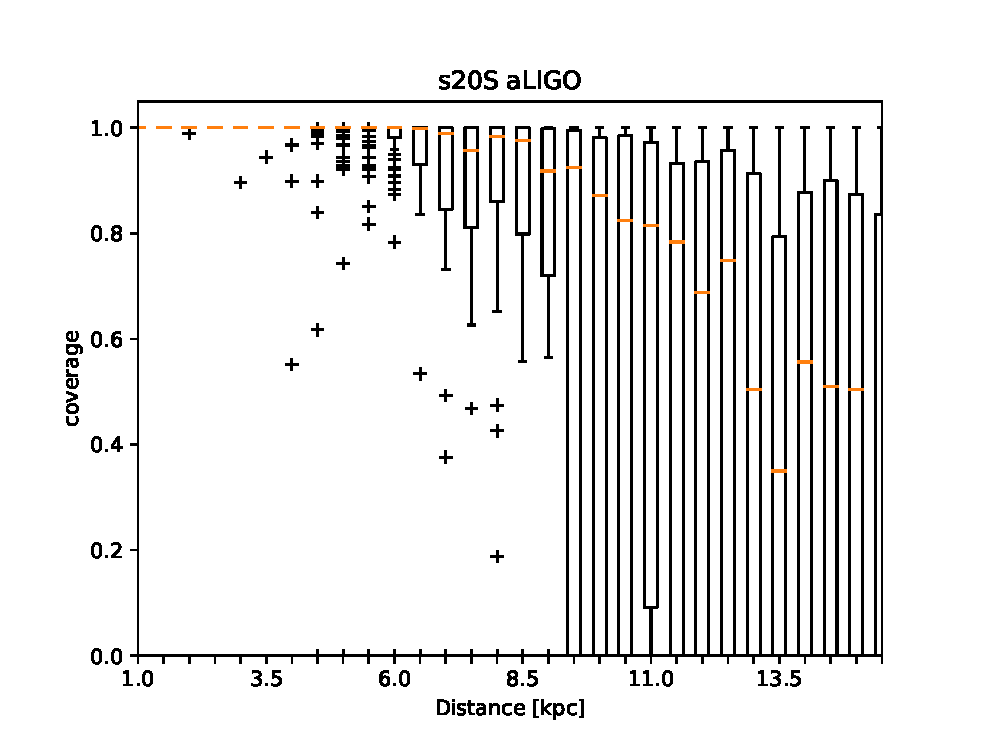
\includegraphics[width=0.5\textwidth]{plots/s20--SFHo_covpbb_boxplot_aLIGO} \\
    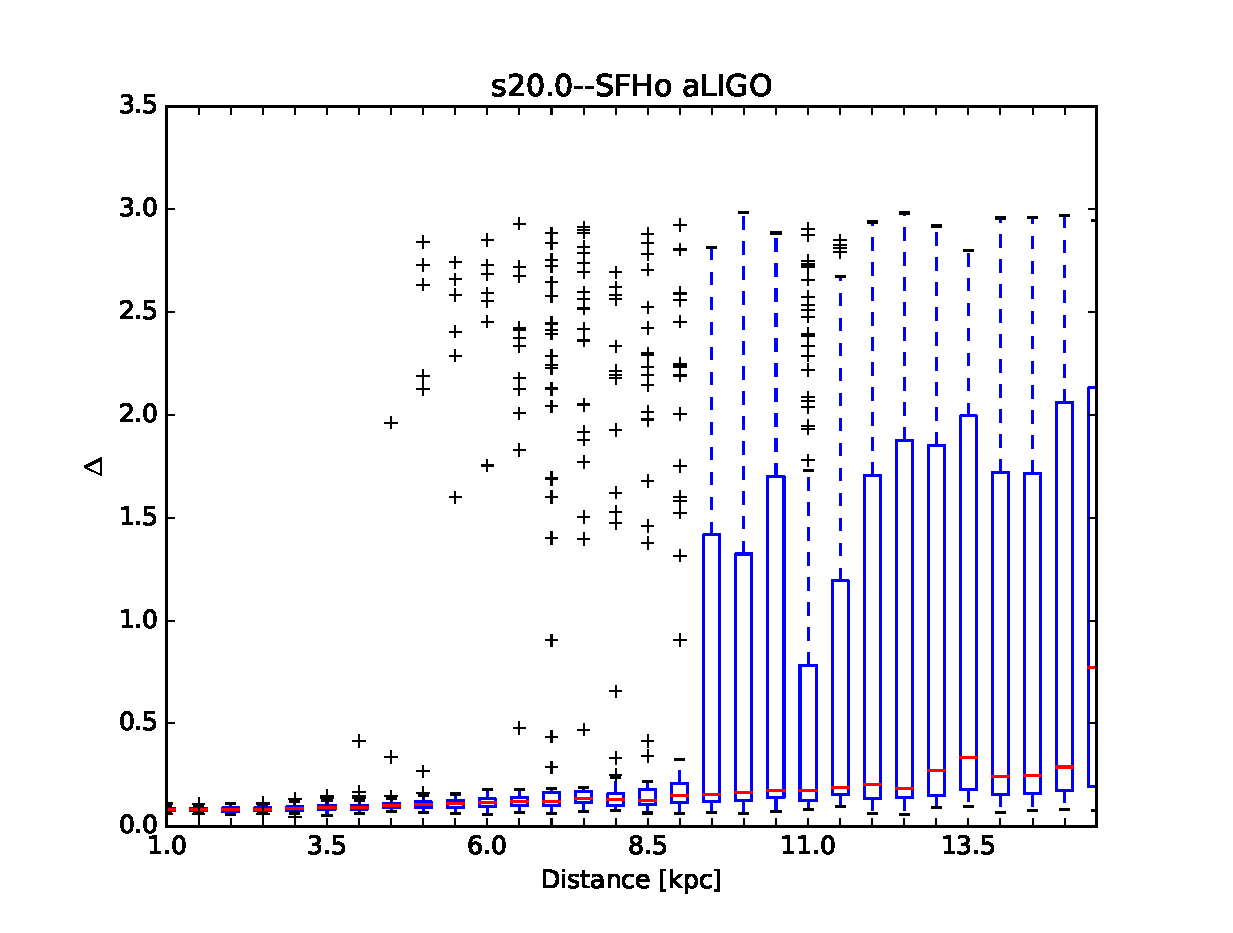
\includegraphics[width=0.5\textwidth]{plots/s20--SFHo_error_boxplot_aLIGO} \\
  \end{tabular}
    
 \caption{Boxplots of $coverage$ (upper panel) and $\Delta$ (lower panel) for {\texttt s20S} signal embedded in aLIGO noise at different distances from the Earth. 100 noise realisations is considered for each distance.} \label{fig:s20results}
\end{figure}


\begin{figure}
 \centering
 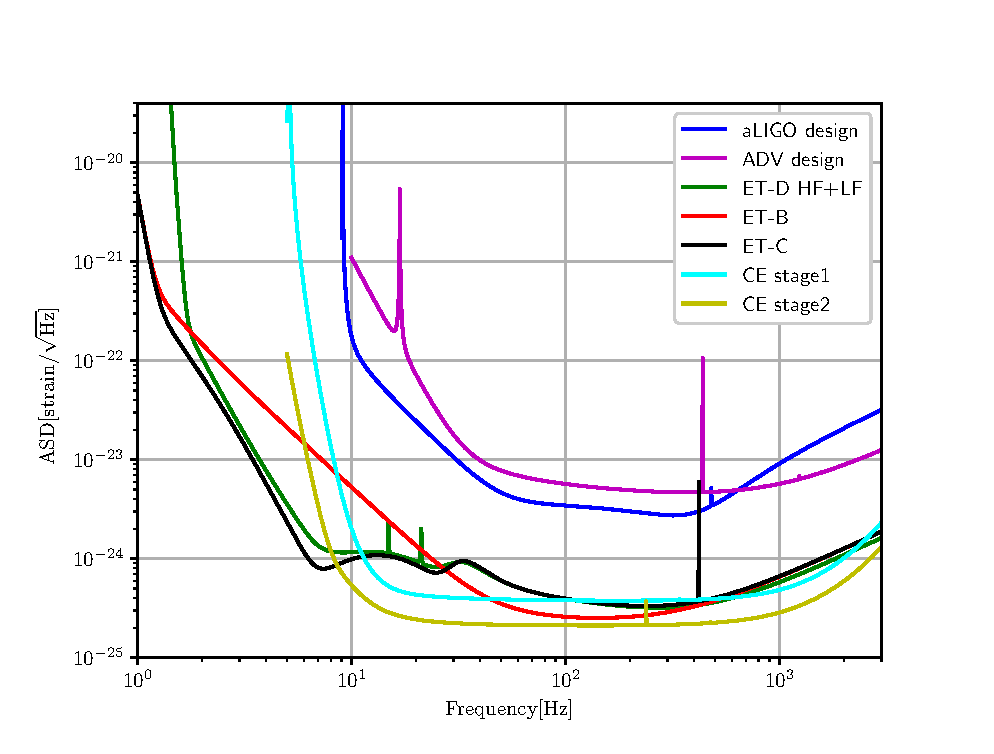
\includegraphics[width=0.5\textwidth]{plots/spectrum}
 \caption{} \label{fig:spectrum}
\end{figure}

\begin{figure}
  \centering
  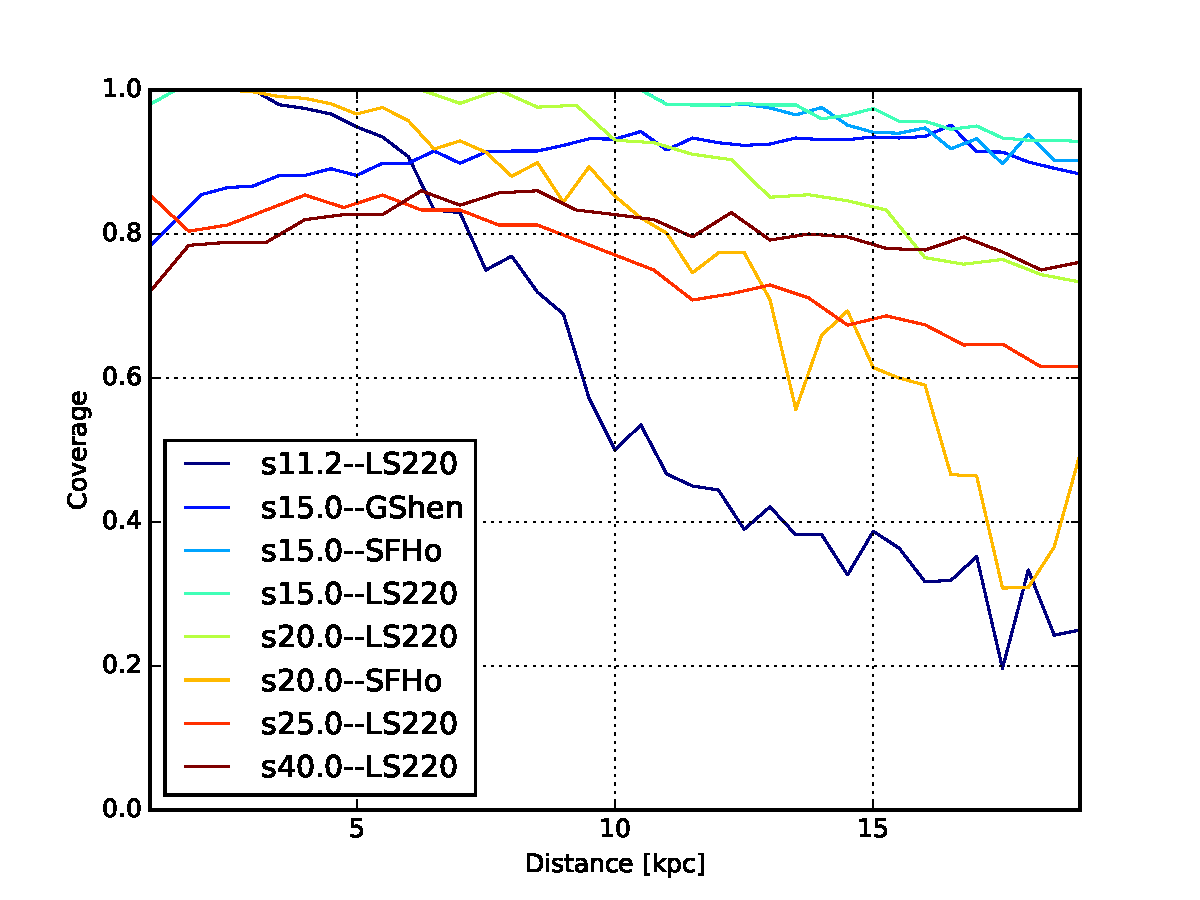
\includegraphics[width=0.5\textwidth]{plots/aLIGO_allwvfs}
 \caption{Median of $coverage$ for 8 CCSN waveforms embedded in aLIGO noise and located at different distance from the Earth. } \label{fig:aLIGOall}
\end{figure}


\begin{table}
  \centering
  \begin{tabular}{c|cccccccc}
    \hline
    
    Simulation & \texttt{s11} & \texttt{s15} & \texttt{s15S} & \texttt{s15G} & \texttt{s20} & \texttt{s20S} & \texttt{s25}  & \texttt{s40}
    \\   
    \hline
    aLIGO      & 19.5         & 55.4         & 59.0          &   60.0        & 34.3         &   35.8          & 116.5         & 98.5
    \\ 
    \hline
    CE2
    \\
    \hline
    ET-B
    \\ 
  \end{tabular}
  \caption{%%
    Matched filter signal-to-noise ratio (SNR) of the simulated waveforms for
    the different GW detectors considered in this study. The source is located
    at 10 kpc and is optimally oriented with respect to the detector.
    %%
  }
  \label{Tab:SNR}
\end{table}
